\section{手写数字及写字人识别实验过程及其结果}
\subsection{样本简介}
\begin{frame}{样本简介}
本论文的手写数字识别实验当中所用的样本分为两类,一类是训练样本集,另一类是
测试样本集。

实验当中的训练样本集采用的是手写数字 MNIST 数据库\parencite{DPMG,kocher99,
cnproceed}。这个数据库当中包含训练集样本 60000 个样例和测试集样本 10000 个
样例。MNIST 数据库当中的数字样本已 经全部大小归一化灰度化并且集中到同一个
固定大小的图像当中。该数据库包括 MST 的 SD-1 和 SD-3 数据库,当中包含一系列
的二级制的手写数字图像。其中 SD-1 的收 集者来源是某高中的在校学生,而 SD-3 
是由人口调查局员工收集的。则我们的训练样 本集也就是 MNIST 当中的训练样本集有 
30000 个样本来自 SD-3,而另外 30000 个样 本来自 SD-1。这 60000 个训练样本
分别来自约 250 个采集者。
\end{frame}

\subsection{Writer Depend类数字识别实验}
\subsubsection{ABCvsA数字识别实验}
\begin{frame}{ABCvsA数字识别实验}
实验内容:以A写字人、B写字人和C写字人,合计3000个数字0到9的数字图像数据为
训练样本集。A写字人的1000个数字0到9的数字图像数据为测试样本集。学习率为1,
单次训练样本数为10个,共训练40次。若识别所得数字与给定的标签匹配,则视为正确;
不匹配则视为错误。

\begin{table}[!hpb]
  \centering
  \caption[指向一个表格的表目录索引]{ABCvsA 数字识别实验结果}
  \label{tab:firstone}
  \begin{tabular}{C{6em}|C{3em}|C{8em}|C{3.5em}} \hline
    训练样本 & ABC     & 样本个数      & 3000 \\ \hline
    测试样本 & A       & 样本个数      & 1000 \\ \hline
    训练次数 & \void   & 单次训练样本数 & 10   \\ \hline
    学习率   & 1       & 正确率        & 99.50\% \\ \hline
  \end{tabular}
\end{table}
\end{frame}

\subsubsection{ABCvsABC 数字识别实验}
\begin{frame}{ABCvsABC 数字识别实验}
实验内容:以 A 写字人、B 写字人和 C 写字人,合计 3000 个数字 0 到 9 的数字
图像数据为总样本集。在总样本集当中随机抽取 2400 个为训练样本集,余下的 600 
个 为测试样本集。学习率为 1,单次训练样本数为 10 个,共训练 40 次。若识别
所得数字 与给定的标签匹配,则视为正确;不匹配则视为错误。

\begin{table}[!hpb]
  \centering
  \caption[指向一个表格的表目录索引]
    {ABCvsABC 数字识别实验结果}
  \label{tab:firstone}
  \begin{tabular}{C{6em}|C{3em}|C{8em}|C{3.5em}} \hline
    训练样本 & ABC     & 样本个数      & 2400     \\ \hline
    测试样本 & A       & 样本个数      & 600      \\ \hline
    训练次数 & 40      & 单次训练样本数 & 10       \\ \hline
    学习率   & 1       & 正确率        & 92.00\% \\ \hline
  \end{tabular}
\end{table}
\end{frame}


\subsection{WriterDepend 类数字识别实验结果分析}
\begin{frame}{WriterDepend 类数字识别实验结果分析}
下面我们选取 Writer Depend 类数字识别实验当中的两个典型的例子 ABCvsA 数字
识别实验以及 MNIST\&ABCvsA 数字识别实验的结果做详细分析。我们从 ABCvsA 
数字识别实验中的训练样本集和测试样本集的手写数字图像样本集当中分别随机抽取
一幅图像如图 \ref{fig:pdfeps-subcaptionbox} 所示。

\begin{figure}[!htp]
  \centering
  \subcaptionbox{实验训练集\label{fig:epspdf:a}} 
  %标题的长度,超过则会换行,如下一个小图。
    {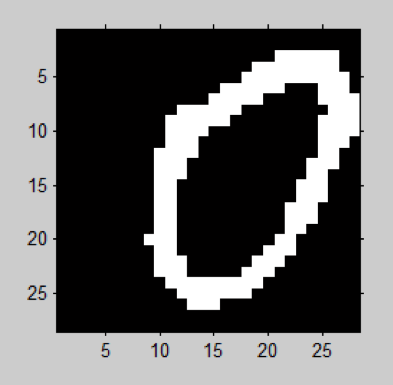
\includegraphics[width=3cm]{figure/experiment1.png}}
  \hspace{4em}
  \subcaptionbox{实验测试集\label{fig:epspdf:b}}
    {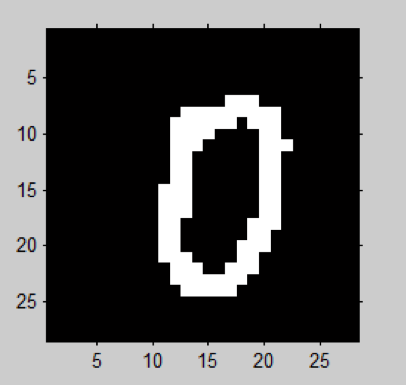
\includegraphics[width=3cm]{figure/experiment2.png}}
  \caption{ABCvsA 数字识别实验集}
  \label{fig:pdfeps-subcaptionbox}
\end{figure}
\end{frame}

\begin{frame}{WriterDepend 类数字识别实验结果分析}
下面我们对上述的训练集和测试集进行 40 次学习率为 2,单次训练样本为 10 的
迭代,得到错误率为 0.50%,而其中每次训练时的误差值组成的历史误差值画图分析
如下:

...
\end{frame}